% ---
\chapter{Fundamentação Teórica}
% ---

A fundamentação teórica a seguir foi elaborada com o objetivo de apresentar os desenvolvimentos conceituais atuais e históricos nesta área, para que seja um ponto de partida para aqueles que estejam iniciando neste estudo. Ao fazê-lo, visamos não apenas ampliar o escopo daqueles capazes de contribuir para esta área, mas também fornecer uma base sólida sobre a qual futuras pesquisas brasileiras possam ser construídas. Esta abordagem é fundamental não só para o enriquecimento do campo, mas também para a construção de uma comunidade acadêmica mais inclusiva e diversificada.

No contexto deste estudo, é fundamental distinguir entre abordagens clássicas e quânticas, assim, utilizaremos o termo ``clássico'' para se referir a sistemas baseados em máquinas tradicionais de silício e seus algoritmos correspondentes, que operam dentro dos paradigmas convencionais da computação. Por outro lado, o termo ``quântico'' será empregado para descrever máquinas e algoritmos que exploram as propriedades da mecânica quântica, tais como superposição e emaranhamento.

Inicialmente será apresentado o conceito de Otimização, depois o formulação matemática do VRP com alguns métodos clássicos de resolução, e por fim, iniciaremos os conceitos introdutórios para a Mecânica Quântica e Computação Quântica.

\section{Problema de Roteamento de Veículos}

O Problema de Roteamento de Veículos (Vehicle Routing Problem – VRP) é um dos problemas de otimização combinatória mais estudados na literatura, sendo frequentemente considerado uma generalização natural do Problema do Caixeiro Viajante (Travelling Salesman Problem – TSP) \cite{gavish1978travelling}. Enquanto o TSP busca determinar a rota mínima para um único agente visitar um conjunto de cidades, o VRP introduz múltiplos veículos e um conjunto mais amplo de restrições operacionais, tornando-o mais adequado para modelar situações reais. Entre essas restrições, destacam-se a capacidade limitada dos veículos, janelas de tempo para atendimento, múltiplos depósitos e custos associados às rotas, o que aumenta significativamente a complexidade do problema.

O problema foi introduzido inicialmente no contexto de distribuição de combustível \cite{dantzig1959truck} e que vem acompanhando o desenvolvimento de métodos computacionais e técnicas de otimização. Houve avanços importantes na formulação matemática do problema especialmente com o uso de programação inteira. Posteriormente, devido a dificuldade computacional associada à sua natureza NP-Difícil \cite{hochba1997approximation}, a área passou a focar em propostas heurística e metaheurísticas capazes de encontrar soluções com boa qualidade em tempo de execução viável, dentre essas propostas podemos destacar: busca tabu \cite{glover1989tabu, glover1990tabu}, algoritmos genéticos \cite{boldberg1989genetic}, simulated annealing \cite{kirkpatrick1983optimization} e colônia de formigas \cite{dorigo2002ant}. 

A relevância do VRP está diretamente relacionada ao seu amplo espectro de aplicações práticas. Problemas de roteamento são centrais em sistemas logísticos modernos, especialmente em contextos como distribuição urbana de mercadorias, coleta de resíduos, transporte escolar e planejamento de rotas para serviços de emergência \cite{golden2008vehicle,toth2002vehicle}. Além disso, com o avanço tecnológico, novas aplicações têm surgido, incluindo o roteamento de drones e veículos autônomos \cite{otto2018optimization}. Nessas aplicações, a eficiência das rotas impacta diretamente custos operacionais, consumo de combustível e emissões de gases poluentes \cite{lin2014survey}, tornando o VRP um problema de grande importância econômica e ambiental.

Ao longo do tempo, diversas variantes do VRP foram propostas para capturar diferentes aspectos do mundo real. Entre as mais estudadas, destacam-se o Problema de Roteamento de Veículos Capacitado (Capacitated VRP – CVRP), no qual cada veículo possui uma capacidade limitada  \cite{solomon1987algorithms}; o VRP com Janelas de Tempo (VRPTW), que considera restrições temporais para atendimento \cite{christofides1979vehicle}; o VRP com Múltiplos Depósitos (MDVRP); e o VRP Estocástico, no qual parâmetros como demanda ou tempo de viagem são incertos \cite{renaud1996tabu, gendreau1996stochastic}. Essas variantes refletem a necessidade de modelos cada vez mais realistas e adaptados a cenários específicos.

Mais recentemente, novas tendências têm emergido na literatura, impulsionadas pela disponibilidade de dados em tempo real e pelo avanço de tecnologias como Internet das Coisas (\textit{Internet of Things} - IoT) e sistemas de posicionamento global (GPS) \cite{ritzinger2016survey, boysen2018scheduling}. Nesse contexto, variantes dinâmicas do VRP têm ganhado destaque, permitindo a adaptação das rotas em tempo real. Além disso, há um crescente interesse em problemas de roteamento sustentáveis, como o VRP verde (Green VRP) \cite{lin2014survey} e o roteamento de veículos elétricos (Electric VRP – EVRP) \cite{schiffer2017electric}, que incorporam preocupações ambientais e restrições energéticas.

Dessa forma, o VRP permanece como um campo de pesquisa ativo e desafiador, com inúmeras aplicações práticas e diversas oportunidades para avanços metodológicos. A complexidade inerente ao problema, aliada à crescente demanda por soluções eficientes e sustentáveis, reforça sua relevância tanto do ponto de vista teórico quanto aplicado \cite{braekers2016vehicle, moghdani2021green}.

\subsection{Formulação Matemática do Problema do Roteamento de Veículos}

Considere um grafo completo\footnote{Um \textit{grafo completo} é aquele em que todo par de vértices distintos está conectado por uma aresta.} $G = (V, E)$, onde $V = \{0, 1, \dots, n\}$ representa o conjunto de vértices, sendo $0$ o depósito e os demais nós correspondentes aos clientes. A cada aresta $(i,j) \in E$ associa-se um custo $c_{ij}$. No VRP capacitado (CVRP), cada cliente $i \in V \setminus \{0\}$ possui uma demanda $d_i$ e cada veículo dispõe de capacidade máxima $Q$ \cite{huang_solving_nodate}. Define-se a variável de decisão binária

\begin{equation}
    x_{ij} =
    \begin{cases}
        1, & \text{se a aresta } (i,j) \text{ é percorrida,} \\
        0, & \text{caso contrário,}
    \end{cases}
\end{equation}

\noindent cuja função objetivo consiste em minimizar o custo total das rotas:

\begin{equation}
    \min \sum_{i \in V} \sum_{\substack{j \in V \\ j \neq i}} c_{ij}\, x_{ij}.
\end{equation}

As restrições do modelo asseguram a viabilidade das rotas. A obrigatoriedade de visita a cada cliente exatamente uma vez é imposta por:

\begin{eqnarray}
\sum_{\substack{j \in V \\ j \neq i}} x_{ij} = 1, & \quad \forall\, i \in V \setminus \{0\}, \\[4pt]
\sum_{\substack{i \in V \\ i \neq j}} x_{ij} = 1, & \quad \forall\, j \in V \setminus \{0\}.
\end{eqnarray}

A conservação de fluxo no depósito, que controla o número de veículos $K$ utilizados, é garantida por:

\begin{eqnarray}
\sum_{j \in V \setminus \{0\}} x_{0j} = K, \\[4pt]
\sum_{i \in V \setminus \{0\}} x_{i0} = K.
\end{eqnarray}

As restrições de capacidade podem ser modeladas por diferentes formulações, frequentemente por meio de variáveis auxiliares ou de estruturas baseadas em fluxo. De forma geral, essas restrições asseguram que a soma das demandas atendidas em cada rota não exceda a capacidade $Q$ do veículo.

Além das restrições de visita, fluxo e capacidade, é necessário garantir a conectividade das rotas, impedindo a formação de sub-rotas desconectadas do depósito. Esse requisito pode ser tratado por diferentes estratégias de modelagem. Uma abordagem clássica consiste no uso de restrições explícitas de eliminação de sub-rotas, dadas por:

\begin{equation}
\sum_{i \in S} \sum_{j \in S} x_{ij} \leq |S| - 1, 
\quad \forall S \subset V,\; 2 \leq |S| \leq |V|-1,
\end{equation}

\noindent que impedem a formação de ciclos em subconjuntos próprios de vértices. Alternativamente, podem ser empregadas formulações baseadas em fluxo, nas quais variáveis adicionais garantem que todo cliente esteja conectado ao depósito por meio de um fluxo viável ao longo das arestas selecionadas.

Outra estratégia amplamente utilizada consiste no uso de variáveis auxiliares, como na formulação de Miller--Tucker--Zemlin (MTZ) \cite{miller1960integer}, na qual $u_i$ representa a carga acumulada no momento da chegada ao nó $i$. Nesse contexto, a variável binária $x_{ij}$ indica se a aresta $(i,j)$ é percorrida, enquanto $d_j$ corresponde à demanda associada ao nó $j$. As restrições são dadas por:

\begin{eqnarray}
u_i - u_j + Q\, x_{ij} \leq Q - d_j, & \quad \forall\, i \neq j,\; i,j \in V \setminus \{0\}, \\[4pt]
d_i \leq u_i \leq Q, & \quad \forall\, i \in V \setminus \{0\}.
\end{eqnarray}

Quando $(i,j)$ é percorrida ($x_{ij}=1$), a restrição implica $u_j \geq u_i + d_j$, induzindo um aumento estrito nos valores de $u$ ao longo da rota. Como consequência, a formação de ciclos desconectados do depósito levaria a uma inconsistência nessas desigualdades, impedindo a ocorrência de sub-rotas. Dessa forma, a formulação assegura simultaneamente o respeito à capacidade $Q$ e a conectividade das rotas.

O TSP pode ser interpretado como um caso particular do VRP no qual há um único veículo ($K = 1$) e as restrições de capacidade são suprimidas — ou, equivalentemente, $Q$ é suficientemente grande para atender todos os clientes em uma única rota. A formulação resultante preserva a mesma função objetivo:

\begin{equation}
    \min \sum_{i \in V} \sum_{\substack{j \in V \\ j \neq i}} c_{ij}\, x_{ij},
\end{equation}

\noindent porém com um conjunto reduzido de restrições. A condição de que cada vértice possua exatamente uma aresta de saída e uma de entrada é expressa por:

\begin{eqnarray}
\sum_{\substack{j \in V \\ j \neq i}} x_{ij} = 1, & \quad \forall\, i \in V, \label{eq:one_out} \\[4pt]
\sum_{\substack{i \in V \\ i \neq j}} x_{ij} = 1, & \quad \forall\, j \in V. \label{eq:one_in}
\end{eqnarray}

A \autoref{eq:one_out} assegura que, após visitar cada vértice, o percurso segue para exatamente um vértice subsequente, enquanto a \autoref{eq:one_in} garante que cada vértice seja visitado exatamente uma vez. Em conjunto, essas restrições impõem a estrutura de grau unitário, prevenindo duplicações e omissões de visitas.

Assim como no VRP, a eliminação de sub-rotas no TSP pode ser tratada por diferentes formulações, incluindo restrições de eliminação de sub-rotas, modelos baseados em fluxo ou o uso de variáveis auxiliares. Em síntese, a transição do VRP para o TSP consiste na remoção das restrições de capacidade e na fixação de um único veículo, reduzindo o problema à determinação de um ciclo hamiltoniano de custo mínimo. Essa relação estrutural evidencia que o TSP constitui um caso particular do VRP, compartilhando a mesma base de modelagem matemática, embora operando sobre um conjunto reduzido de restrições.

\section{Introdução a Mecânica Quântica e Computação Quântica}
\subsection{Mecânica Quântica}

\textcite{Schuld2021} afirma que os computadores são dispositivos físicos baseados em circuitos eletrônicos que processam informações. Embora os processos físicos envolvam partículas macroscópicas e/ou atômicas/subatômicas, como elétrons, átomos e moléculas, podemos descrevê-los utilizando métodos da teoria das probabilidades e estatística. Em particular, aplicamos conceitos matemáticos para lidar com grandes populações e aproximações na solução de problemas físicos. Por exemplo, utilizamos uma teoria clássica e macroscópica das propriedades eletrônicas para a construção de circuitos que executam tarefas. No entanto, os sistemas microscópicos, como fótons, elétrons e átomos, requerem uma outra descrição matemática, conhecida como \textit{teoria quântica}.


Para compreender minimamente a teoria quântica é necessário uma revisão de conceitos de Álgebra Linear. Para isso, \textcite{Almeida2020} nos apresenta uma metodologia satisfatória para introduzir esses conceitos e outros, como \textit{kets} e \textit{bras}, tão comuns na teoria quântica, também é importante conhecer os conceitos de incerteza, superposição e emaranhamento \cite{hewitt2000fundamentos, mahon2000mecanica}. 

Iniciando com espaço vetorial no corpo dos reais um vetor de $n$ dimensões pode ser representado, de forma linear quanto matricial, por
$$
    \vec{v} = v_1\vec{b_1}+v_2\vec{b_2}+\ldots+v_n\vec{b_n}=\left[\vec{b_1}, \vec{b_2},\cdots, \vec{b_n}\right]\left[\begin{array}{c}
         v_1\\
         v_2\\ 
         \vdots\\
         v_n
    \end{array}\right];\ v_1, v_2,\ldots, v_n \in \R
$$

Sendo $\left[\vec{b_1}, \vec{b_2},\dots, \vec{b_n}\right]$ uma base ortonormal para o espaço vetorial $\R^n$, podemos representar o vetor $\vec{v}$ de forma única tal como:
\begin{equation}
    \label{eq:vetor_v_em_R}
    \vec{v}=\left[\begin{array}{c}
         v_1\\
         v_2\\ 
         \vdots\\
         v_n
    \end{array}\right];\quad v_1, v_2,\ldots, v_n \in \R
\end{equation} 

Nos conceitos de Mecânica Quântica um vetor em $\C^n$, é representado, semelhante a \autoref{eq:vetor_v_em_R}
$$
    \label{eq:vetor_em_C}
    \ket{\varphi} = \left[\begin{array}{c}
         z_0 \\
         z_1 \\
         \vdots \\
         z_{n-1}
    \end{array}\right];\quad z_0,z_1,\ldots, z_{n-1}\in\C
$$

O simbolismo proposto por \textcite{dirac1981principles} para tratar dos conceitos de Mecânica Quântica apresenta a notação deum vetor de estado ser dado pelo símbolo $\ket{\ }$, que se pronuncia \textit{ket} e um elemento do espaço dual ser denotado por $\bra{\ }$, que se pronuncia por \textit{bra}. Assim, como exemplo, o vetor $\ket{\varphi}$ é lido como ``\textit{ket} $\varphi$'' e o vetor dual $\bra{\varphi}$ é lido como ``\textit{bra} $\varphi$''. Veja que se tomarmos, como um exemplo, $n=2$ teremos então que $\ket{\varphi}\in\C^2$ e $a,b\in\C$ então
\begin{equation}\label{eq:varphi_matricial}
    \ket{\varphi}=a\left(\begin{array}{c}
         1 \\ 
         0
    \end{array}\right)+b\left(\begin{array}{c}
         0 \\
         1
    \end{array}\right)
\end{equation}

Observe que os vetores $\left(\begin{array}{c}
         1 \\ 
         0
    \end{array}\right)$ e $\left(\begin{array}{c}
         0 \\
         1
    \end{array}\right)$ formam uma base para $\C^2$, com isso é possível definir esses vetores como sendo
\begin{equation}\label{eq:varphi_ket_notation}
\left(\begin{array}{c}
     1 \\
     0
\end{array}\right)=\ket{0}\text{ e }\left(\begin{array}{c}
     0 \\
     1
\end{array}\right)=\ket{1}
\end{equation}
com isso a \autoref{eq:varphi_matricial} com a \autoref{eq:varphi_ket_notation} temos:
$$\ket{\varphi}=a\ket{0}+b\ket{1}$$
    
Mudanças de estado quânticos são transformações lineares de $\C^n\Rightarrow \C^m$. Uma transformação linear é uma função entre dois espaços vetoriais que preserva as operações de adição vetorial e multiplicação por escalar, ou seja, se $T$ é uma transformação linear, $T:\V[n]\rightarrow\V[m]$, onde $\V[n]
$ é um espaço vetorial com $n$ entradas (dimensão $n$) e $\V[m]$ é um espaço vetorial com $m$ entradas (dimensão $m$), $T$ preserva
\begin{enumerate}
    \item $T(\ket{\phi}+\ket{\psi}) = T(\ket{\phi})+T(\ket{\psi})$
    \item $T(z\ket{\phi})=zT(\ket{\phi})$, $\forall z\in\C$
\end{enumerate}

Quando a transformação linear $T:\V\rightarrow\V$ é dito que $T$ é um \textit{operador linear}. Uma transformação linear, por conveniência, pode ser representada por uma matriz, o que possibilita a utilização de conceitos de operações entre matrizes e relacioná-las às transformações lineares \cite{dettman1986introduction}.

Na computação clássica, a unidade básica de memória é chamada de \textit{bit}, que pode assumir valores entre 0 e 1. Um bit é o potencial elétrico nulo (ou baixo) representado pelo 0 e o potencial elétrico alto representado pelo 1. Na computação quântica a unidade básica de memória é o \textit{qubit} que é representado por um vetor bidimensional de norma 1 e os estados\footnote{O termo estado pode sempre ser identificado como sendo um vetor de norma 1 e pode ser visto como o ``valor'' do qubit antes da medição} de um qubit correspondentes aos valores 0 e 1 são $\ket{0}$ e $\ket{1}$. A coexistência quântica é representada matematicamente por
    \begin{equation}
        \label{eq:estados_superposicao}
        \ket{\phi}=\alpha_0\ket{0}+\alpha_1\ket{1}
    \end{equation}
    onde $\alpha_0, \alpha_1\in\C$ que obedecem a
    $$
        |\alpha_0|^2+|\alpha_1|^2=1
    $$
    
Os números complexos $\alpha_0$ e $\alpha_1$ são chamados de \textit{amplitude} do estado $\ket{\phi}$. A coexistência dos bits 0 e 1 não podem ser implementada em um sistema computacional clássico, pois não é possível obter um estado baixo e alto ao mesmo tempo, porém na mecânica quântica, é possível ter sistemas com potencial baixo e alto ao mesmo tempo, definido como \textit{superposição}. Matematicamente, um estado em superposição é uma combinação linear dos estados básicos, tal como por exemplo $\ket{0}$ e $\ket{1}$ apresentados na \autoref{eq:estados_superposicao} \cite[pág. 13]{nielsen_quantum_2002}.
    
    % \*n se usa a primeira pessoa do plural neste tipo de texto, mas sempre a terceira do singular. Por exemplo: "É possível decompor..."*\
    É possível decompor unicamente o amplitude complexa de $\alpha$ como um produto $e^{i\theta}|\alpha|$, onde $|\alpha|$ é um numero real não-negativo correspondente a magnitude $\alpha$, e $e^{i\theta}=\frac{\alpha}{|\alpha|}$ tem norma 1, o valor $\theta$ é conhecido como \textit{fase} e podemos nos referir a $e^{i\theta}$ como um \textit{fator de fase} \cite{Rieffel2000}.
    
    O estado de um qubit pode ser caracterizado por dois ângulos $\theta$ e $\varphi$ de forma:
    $$
        \label{eq:ket_psi}
        \ket{\psi}=\cos\left(\dfrac{\theta}{2}\right)\ket{0}+e^{i\varphi}\sen\left(\dfrac{\theta}{2}\right)\ket{1}
    $$
onde $0\leq\theta\leq\pi$ e $0\leq\varphi\leq2\pi$, o que mostra que existe uma relação entre o conjunto de estados de 1 qubit e pontos na superfície de uma esfera de raio 1, denominada de \textit{esfera de Bloch}, como apresentado na \autoref{fig:esfera_de_bloch}.
    

\begin{figure}[!htb]
    \centering
    \caption{Esfera de Bloch para $\ket{\psi}$}    
    \label{fig:esfera_de_bloch}
\begin{tikzpicture}[line cap=round, line join=round, >=Triangle]
  \clip(-2.19,-2.49) rectangle (2.66,2.58);
  \draw [shift={(0,0)}, lightgray, fill, fill opacity=0.1] (0,0) -- (56.7:0.4) arc (56.7:90.:0.4) -- cycle;
  \draw [shift={(0,0)}, lightgray, fill, fill opacity=0.1] (0,0) -- (-135.7:0.4) arc (-135.7:-33.2:0.4) -- cycle;
  \draw(0,0) circle (2cm);
  \draw [rotate around={0.:(0.,0.)},dash pattern=on 3pt off 3pt] (0,0) ellipse (2cm and 0.9cm);
  \draw (0,0)-- (0.70,1.07);
  \draw [->] (0,0) -- (0,2);
  \draw [->] (0,0) -- (-0.81,-0.79);
  \draw [->] (0,0) -- (2,0);
  \draw [dotted] (0.7,1)-- (0.7,-0.46);
  \draw [dotted] (0,0)-- (0.7,-0.46);
  \draw (-0.08,-0.3) node[anchor=north west] {$\varphi$};
  \draw (0.01,0.9) node[anchor=north west] {$\theta$};
  \draw (-1.01,-0.72) node[anchor=north west] {$x$};
  \draw (2.07,0.3) node[anchor=north west] {$y$};
  \draw (-0.5,2.6) node[anchor=north west] {$\ket{0}$};
  \draw (-0.4,-2) node[anchor=north west] {$\ket{1}$};
  \draw (0.4,1.65) node[anchor=north west] {$\ket{\psi}$};
  \scriptsize
  \draw [fill] (0,0) circle (1.5pt);
  \draw [fill] (0.7,1.1) circle (0.5pt);
\end{tikzpicture}
\fonte{Própria, 2024}
\end{figure}

  % \subsection{Portas Lógicas Quânticas}\label{sec:portas_logicas}
    
    Portas lógicas quânticas são transformações lineares $T:\C^n\rightarrow\C^n$, ou seja, são operadores lineares, isto é, portas lógicas para 1 qubit é uma matriz quadrada bidimensional unitária. Por exemplo, a porta Hadamard:
    $$
        \label{eq:hadamard}
        H=\dfrac{1}{\sqrt{2}}\left[\begin{array}{cc}
             1 & 1 \\
             1 & -1
        \end{array}\right]
    $$
    
    Aplicando a porta Hadamard ao vetor $\ket{0}$, obtemos:
    $$
        \label{eq:aplicacao_hadamard_0}
        H\ket{0}=H\left[\begin{array}{c}
             1 \\
             0
        \end{array}\right] = \dfrac{1}{\sqrt{2}}\left[\begin{array}{cc}
             1 & 1 \\
             1 & -1
        \end{array}\right]\left[\begin{array}{c}
             1 \\
             0
        \end{array}\right]=\dfrac{1}{\sqrt{2}}\left[\begin{array}{c}
             1 \\
             1
        \end{array}\right]=\dfrac{1}{\sqrt{2}}\ket{0}+\dfrac{1}{\sqrt{2}}\ket{1}
    $$
    
Perceba que o vetor resultante tem norma 1 e podemos denotar esse vetor por $\ket{+}$, isto é
    $$
        \label{eq:ket_mais}
        \ket{+}=\dfrac{1}{\sqrt{2}}\ket{0}+\dfrac{1}{\sqrt{2}}\ket{1}
    $$
    
    Ao aplicar a porta Hadamard no vetor $\ket{1}$ resulta em
    $$
        \label{eq:aplicacao_hadamard_1}
        H\ket{1}=H\left[\begin{array}{c}
             0\\
             1
        \end{array}\right] = \dfrac{1}{\sqrt{2}}\left[\begin{array}{cc}
             1 & 1 \\
             1 & -1
        \end{array}\right]\left[\begin{array}{c}
             0\\
             1
        \end{array}\right]=\dfrac{1}{\sqrt{2}}\left[\begin{array}{c}
             1 \\
             -1
        \end{array}\right]=\dfrac{1}{\sqrt{2}}\ket{0}-\dfrac{1}{\sqrt{2}}\ket{1},
    $$
que pode ser denotado por $\ket{-}$, isto é, 

    $$
        \ket{-}=\dfrac{1}{\sqrt{2}}\ket{0}-\dfrac{1}{\sqrt{2}}\ket{1}
    $$
    
    Outras portas lógicas podem ser apresentadas:
    \begin{enumerate}
    \begin{minipage}{0.5\textwidth}
        \item Identidade
        $$
            id=\left[\begin{array}{cc}
                 1 & 0 \\
                 0 & 1
            \end{array}\right]
        $$
    \end{minipage}
    \begin{minipage}{0.5\textwidth}
        \item Matriz de \textit{Pauli X}
        $$
            X=\left[\begin{array}{cc}
                 0 & 1 \\
                 1 & 0
            \end{array}\right]
        $$
    \end{minipage}
    \begin{minipage}{0.5\textwidth}
        \item Matriz de \textit{Pauli Y}
        $$
            X=\left[\begin{array}{cc}
                 1 & -i \\
                 i & 0
            \end{array}\right]
        $$
    \end{minipage}
    \begin{minipage}{0.5\textwidth}
        \item Matriz de \textit{Pauli Z}
        $$
            Z=\left[\begin{array}{cc}
                 1 & 0 \\
                 0 & -1
            \end{array}\right]
        $$
    \end{minipage}
    \begin{minipage}{0.5\textwidth}
        \item Porta fase
        $$
            S=\left[\begin{array}{cc}
                 1 & 0 \\
                 0 & i
            \end{array}\right]
        $$
    \end{minipage}
    \begin{minipage}{0.5\textwidth}
        \item Porta fase conjugada
        $$
            S^{\dagger}=\left[\begin{array}{cc}
                 1 & 0 \\
                 0 & -i
            \end{array}\right]
        $$
    \end{minipage}
    \begin{minipage}{0.5\textwidth}
        \item Porta $\pi/8$ ou Porta $T$
        $$
            T=\left[\begin{array}{cc}
                 1 & -i \\
                 i & e^{\frac{i\pi}{4}}
            \end{array}\right]
        $$
    \end{minipage}
    \begin{minipage}{0.5\textwidth}
        \item Porta $\pi/8$ conjugada ou Porta $T$ \\   
        conjugada
        $$
            T^{\dagger}=\left[\begin{array}{cc}
                 1 & -i \\
                 i & e^{-\frac{i\pi}{4}}
            \end{array}\right]
        $$
    \end{minipage}
    \end{enumerate}
    
A matriz transposta conjugada é denotada pelo símbolo ``$\dagger$''. Podemos reescrever os números complexos, utilizando a fórmula de Euler:
    $$
        e^{\pm\frac{i\pi}{4}} = \dfrac{1\pm i}{\sqrt{2}}
    $$
    
Interessante notar que as portas quânticas são reversíveis, como por exemplo para qualquer $\ket{\phi}$ teremos:
    $$
        H\otimes H\ket{\phi} = \ket{\phi}.
    $$
    
De fato, pois tomando $\ket{\phi}=\left[\begin{array}{c}
         \alpha \\
         \beta
    \end{array}\right]$ teremos
    $$
        H\ket{\phi}= \dfrac{1}{\sqrt{2}} \left[\begin{array}{cc}
             1 & 1 \\
             1 & -1
        \end{array}\right]\left[\begin{array}{c}
             \alpha \\
             \beta
        \end{array}\right] = \left[\begin{array}{c}
             \dfrac{1}{\sqrt{2}}(\alpha+\beta) \\
             \dfrac{1}{\sqrt{2}}(\alpha - \beta)
        \end{array}\right].
    $$
    
    Com isto
    $$
        H\otimes H\ket{\phi}= \dfrac{1}{\sqrt{2}}\left[\begin{array}{cc}
             1 & 1 \\
             1 & -1 
        \end{array}\right]\left[\begin{array}{c}
             \dfrac{1}{\sqrt{2}}(\alpha+\beta) \\
             \dfrac{1}{\sqrt{2}}(\alpha - \beta)
        \end{array}\right] = \left[\begin{array}{c}
             \alpha \\
             \beta 
        \end{array}\right]=\ket{\phi}.
    $$
    
    
Como dito no início do capítulo, quaisquer portas lógicas quânticas são matrizes quadradas bidimensionais unitárias e \textcite[pag. 425]{Anton2012} apresenta a seguinte \autoref{def:matriz_hermetiana}:

    \begin{defi}
        \label{def:matriz_hermetiana}
        Uma matriz quadrada complexa $A$ é dita \textbf{unitária} se $$A^{-1}=A^*,$$ onde $A^*$ representa o complexo conjugado da matriz $A$ e $A^{-1}$ a matriz inversa de $A$ e é dita \textbf{hermitiana} se $$A^*=A$$
    \end{defi}
    
Sendo assim, a $UU=I_n$, onde $U$ é a matriz de transformação equivalente a uma porta quântica e $I_n$ é a matriz identidade de ordem $n$.

% {\color{red} (Novo - Continuação do Relatório)}

    % \subsection{Estados Quânticos de 2 ou mais qubits}
Como visto anteriormente 1 qubit é representado por um vetor bidimensional de norma 1 e os seus estados correspondem aos valores $\ket{0}$ ou $\ket{1}$, e \textcite{Amaral2011MecanicaFormacao} diz que dois qubits podem assumir quatro valores entre 00, 01, 10 e 11 que correspondem a um sistema quântico de 4 níveis e seus estados serão respectivamente $\ket{00}, \ket{01}, \ket{10}$ e $\ket{11}$, assim qualquer $\ket{\psi}$ é uma superposição escrita da forma:
    $$
        \ket{\psi}=\alpha_{00}\ket{00}+\alpha_{01}\ket{01}\alpha_{10}\ket{10}\alpha_{11}\ket{11},
    $$
onde $\alpha_{00}, \alpha_{01}, \alpha_{10}, \alpha_{11}\in\C$. A medição resultará em algum estado apresentado de forma exclusiva e estocástica, isso significa que não há forma de saber o resultado da medição mesmo conhecendo $\ket{\psi}$, mas se é conhecido então sabemos suas probabilidades \cite{Marquezino2019}, que serão 
    $$
        \begin{array}{lcl}
             \text{prob}(00) & = &|\alpha_{00}|^2 \\
             \text{prob}(01) & = &|\alpha_{01}|^2 \\
             \text{prob}(10) & = &|\alpha_{10}|^2 \\
             \text{prob}(11) & = &|\alpha_{11}|^2 \\
        \end{array} 
    $$
    
    Com isso, apenas uma única medição não possibilita determinar $\ket{\psi}$, então é necessário gerar $\ket{\psi}$ novamente e refazer as medições, mas mesmo assim, ainda não será possível determinar o estado exatamente.
   
    Na referência \textcite{Marquezino2019} encontramos que para determinar o estado $\ket{\psi}$ de 2 qubits se $\ket{\psi}$ for um dos estados de base computacional então sabemos o estado de cada qubit, pois tomando como exemplo o estado $\ket{\psi}=\ket{10}$ fatoramos da seguinte forma:
    $$
        \ket{10}=\ket{1}\otimes\ket{0}=\ket{1}\ket{0}
    $$
    onde $\otimes$ é chamado de \textit{produto de Kronecker} e sua operação esta descrito na \autoref{def:kronecker}.
    \begin{defi}\label{def:kronecker}
       Seja $A$ uma matriz $m\times n$ e $B$ uma matriz $p\times q$, a operação $\otimes$ entre $A$ e $B$ é dada da seguinte forma:
       \begin{align*}
           A\otimes B & =\left[\begin{array}{ccc}
                a_{11}B & \cdots & a_{1n}B \\
                \vdots & \ddots & \vdots \\
                a_{m1}B & \cdots & a_{mn}B
           \end{array}\right] \\&
          = \left[\begin{array}{ccc}
                a_{11}\left[\begin{array}{ccc}
                b_{11} & \cdots & b_{1q} \\
                \vdots & \ddots & \vdots \\
                b_{p1} & \cdots & b_{pq}
           \end{array}\right]   & \cdots & a_{1n}\left[\begin{array}{ccc}
                b_{11} & \cdots & b_{1q} \\
                \vdots & \ddots & \vdots \\
                b_{p1} & \cdots & b_{pq}
           \end{array}\right]  \\
                \vdots & \ddots & \vdots \\
                a_{m1}\left[\begin{array}{ccc}
                b_{11} & \cdots & b_{1q} \\
                \vdots & \ddots & \vdots \\
                b_{p1} & \cdots & b_{pq}
           \end{array}\right]  & \cdots & a_{mn}\left[\begin{array}{ccc}
                b_{11} & \cdots & b_{1q} \\
                \vdots & \ddots & \vdots \\
                b_{p1} & \cdots & b_{pq}
           \end{array}\right] 
           \end{array}\right] \\&
          = \left[\begin{array}{ccccccc}
                a_{11}b_{11} & \cdots & a_{11}b_{1q} &  & a_{1n}b_{11} & \cdots & a_{1n}b_{1q} \\
                \vdots & \ddots & \vdots & \cdots & \vdots & \ddots & \vdots \\
                a_{11}b_{p1} & \cdots & a_{11}b_{pq} &  & a_{1n}b_{11} & \cdots & a_{1n}b_{pq}\\
                & \vdots &  & \ddots &  & \vdots &  \\
                a_{m1}b_{11} & \cdots & a_{m1}b_{1q} &  & a_{mn}b_{11} & \cdots & a_{mn}b_{1q}\\
                \vdots & \ddots & \vdots & \cdots & \vdots & \ddots & \vdots \\
                a_{m1}b_{p1} & \cdots & a_{m1}b_{pq} &  & a_{mn}b_{11} & \cdots & a_{mn}b_{pq}\\
           \end{array}\right].
        \end{align*}
    \end{defi}
   \noindent observe que a matriz resultante tem dimensão $mp\times nq$. Assim com a \autoref{def:kronecker} teremos que, por exemplo, para $\ket{10}$ o vetor resultante é apresentado na \autoref{eq:produto_externo_ket_10}.
   \begin{equation}
       \ket{10} =\ket{1}\otimes\ket{0}=\left[\begin{array}{c}
            0 \\
            1
       \end{array}\right] \otimes \left[\begin{array}{c}
            1 \\
            0
       \end{array}\right] = \left[\begin{array}{cc}
            0 \left[\begin{array}{c}
            1 \\
            0
       \end{array}\right]\\ \\
            1 \left[\begin{array}{c}
            1 \\
            0
       \end{array}\right]
       \end{array}\right] = \left[\begin{array}{c}
            0 \\
            0 \\
            1 \\
            0 \\
       \end{array}\right].
       \label{eq:produto_externo_ket_10}
   \end{equation}
   
   Desta forma, podemos generalizar para uma base $n$ ortonormal teremos que o estado $\ket{\psi}=\ket{\alpha_1\dots\alpha_n}$ para $\alpha_i\in \{0,1\}\ (i=1,\hdots,n)$, será da forma:
   $$
       \ket{\psi}=\ket{\alpha_1\hdots\alpha_n}=\ket{\alpha_1}\otimes\hdots\otimes\ket{\alpha_n}.
   $$
   
   Um sistema quântico composto pode estar em um estado onde suas partes não tem um estado definido, como por exemplo, para encontrar o estado de 1 qubit de $\ket{\psi_1}=\alpha\ket{0}+\beta\ket{1}$ e $\ket{\psi_2}=\gamma\ket{0}+\delta\ket{1}$ de tal forma que
   $$
       \dfrac{\ket{00}+\ket{11}}{\sqrt{2}}=(\alpha\ket{0}+\beta\ket{1})\otimes(\gamma\ket{0}+\delta\ket{1}),
   $$
   teremos que $\alpha\gamma = \frac{1}{\sqrt{2}}, \alpha\delta=0, \beta\gamma=0$ e $\beta\delta=\frac{1}{\sqrt{2}}$ e esse sistema não admite nenhuma solução, sendo assim o estado $\ket{\psi}$ de 2 qubits não pode ser descrito como um produto de Kronecker de 1 qubit. 
   
    % Para \cite{Marquezino2019} um estado emaranhado é definido por um sistema composto que não pode ser fatorado pelo produto de Kronecker, isto é, enquanto que em um circuito booleano um estado está definido entre 0 e 1 em cada junção de porta, nem sempre é verdade para um estado quântico \cite{lipton_quantum_2014}.
    Um estado emaranhado é definido por um sistema composto que não pode ser fatorado pelo produto de Kronecker, isto é, enquanto que em um circuito booleano um estado está definido entre 0 e 1 em cada junção de porta, nem sempre é verdade para um estado quântico \cite{Marquezino2019, lipton_quantum_2014}.
   
\subsection{Computação Quântica}

A computação é o processo sistemático de manipular e processar informações utilizando recursos computacionais, tais como dispositivos eletrônicos e algoritmos, com o objetivo de realizar tarefas específicas, resolver problemas ou tomar decisões. Isso envolve não apenas a manipulação de dados, mas também a execução de instruções lógicas e matemáticas, a fim de transformar esses dados em resultados úteis e significativos para os usuários.

Não se espera que um Computador Quântico (\textit{Quantum Computing} - QC) sejam classicamente simuláveis e para obter vantagem sobre as abordagens clássicas é necessário implementar um codificador que seja difícil de ser simulado classicamente \cite{havlicekSupervisedLearningQuantumenhanced2019}. \textcite{Schuld_Petruccione_2018} afirma que existem diferentes maneiras de codificar uma informação clássica em um sistema quântico tal como codificação de base, codificação de amplitude e outras formas. A codificação de base é a forma mais direta de cálculo, que associa uma base de estado de um sistema de $n$-qubits em uma cadeia de bits clássicos, por exemplo o estado $\ket{3}=\ket{0011}$ é associado a cadeia clássica $(0011)$. Codificação de amplitude é menos comum na computação quântica, que associa um vetor real com uma amplitude quântica, a normalização clássica de vetor de forma que $x\in\C^{2^n}, \sum_k|x_k|^2=1$ pode representar a  amplitude de um estado quântico $\ket{\psi}=\displaystyle\sum_{j=1}^{2^n}x_j\ket{j}$.


\textcite{houssein_machine_2022} apresenta uma divisão de categorias sobre a integração de algoritmos clássicos e quânticos como mostrado na \autoref{fig:category_quantum_classical_algorithm}.

\begin{figure}[!htb]
    \centering
    \caption{Integração de algoritmos e dados quânticos e clássicos.}
    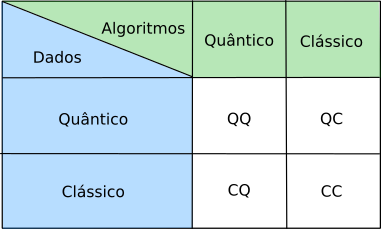
\includegraphics[scale=1]{figs/quadro_quantico_classico.png}
    \label{fig:category_quantum_classical_algorithm}
    \fonte{Própria, baseada em \cite{houssein_machine_2022}, 2024.}
\end{figure}

Atualmente os computadores quânticos estão marcados por realizarem cálculos quânticos de maneira limitada e sujeita a ruídos, assim como outras restrições. Denominado era Quântica de Escala Intermediária e Ruidosa (NISQ) como sendo o período de transição entre os estágios iniciais experimentais da computação quântica e a futura era tolerante a falhas e que podem realizar operações complexas e precisas em escala muito maior 
\cite{Lau_Lim_Shrotriya_Kwek_2022}, são dificuldades a serem superadas com os avanços na área. As principais características dos computadores quântico da era NISQ são:
\begin{enumerate}
    \item \textbf{Capacidade Limitada}: não são capazes de cálculos em grande escala ou altamente complexos;
    \item \textbf{Erros e Ruídos}: apesar de serem capazes de realizar cálculos, estes podem ser afetados por erros introduzidos pela interação do sistema quântico com o ambiente externo o que pode levar à decoerência e a outros tipos de erro;
    \item \textbf{Número de qubits}: possui quantidade de qubits que não podem ser simulados de forma eficiente por computadores clássicos, mas ainda não têm qubits suficientes para permitir correção de erros eficaz e computação à prova de falhas;
    \item \textbf{Computação sem Correção de Erro}: os computadores operam sem correção de erros quânticos completos, limitando a complexidade e precisão dos cálculos que podem realizar.
\end{enumerate}

\subsubsection{Computação Quântica de Variáveis Contínuas}

A QC fundamenta-se nas propriedades estatísticas das partículas 
subatômicas, classificadas em duas categorias fundamentais: férmions e bósons \cite{cohen2019quantum}. Os férmions obedecem ao Princípio de Exclusão de Pauli, que impede que duas partículas ocupem simultaneamente o mesmo estado quântico;  essa característica confere-lhes um caráter naturalmente discreto, tornando-os  a base conceitual dos computadores quânticos convencionais baseados em qubits \cite{sakurai2020modern}.

Em contrapartida, os bósons podem ocupar o mesmo estado quântico simultaneamente.  O exemplo mais proeminente são os fótons, que podem ser descritos matematicamente  como osciladores harmônicos quânticos possuidores de infinitos níveis de energia  \cite{braunstein2005quantum}. Essa propriedade permite a codificação de uma vasta quantidade de informação em um único sistema físico, possibilitando estratégias de correção de erros quânticos potencialmente mais eficientes e compactas — como os códigos Gottesman-Kitaev-Preskill (GKP) — do que a abordagem tradicional baseada em grandes redes de múltiplos qubits interligados \cite{gottesman2000encoding, weedbrook2012gaussian}.

A Computação Quântica de Variáveis Contínuas (\textit{Continuous Variables Quantum Computing} - CVQC) processa informação não em bits binários, mas em estados que podem assumir qualquer valor dentro de um intervalo contínuo \cite{braunstein2005quantum}, como amplitudes e fases de campos eletromagnéticos. Analogamente, enquanto a QC convencional opera como um interruptor de luz --- transitando entre estados discretos com suas superposições ---, a CVQC opera como um dimmer \cite{lloyd1999quantum}, capaz de ajustar o brilho a qualquer nível dentro de uma faixa contínua.

O estado de um sistema de CVQC é descrito no espaço de fase por dois observáveis conjugados denominados quadraturas: a posição ($\hat{x}$), associada à amplitude do campo, e o momento ($\hat{p}$), associado à sua fase. Sujeitas ao Princípio da Incerteza de Heisenberg, essas variáveis não podem ser determinadas simultaneamente com precisão arbitrária \cite{serafini_quantum_2023, weedbrook2012gaussian}. Nesse paradigma, a unidade fundamental de informação não é o \textit{qubit}, mas o \textit{qumode} (modo quântico), que habita um espaço de Hilbert de dimensão infinita \cite{lloyd1999quantum}. A CVQC bosônica figura entre as abordagens mais promissoras para a computação tolerante a falhas: 
em vez de controlar individualmente milhares de átomos ou íons, pulsos de luz são ``moldados'' em estados quânticos complexos --- como os estados de gato de Schrödinger ou os códigos GKP --- intrinsecamente mais robustos contra ruídos e decoerência ambiental \cite{gottesman2000encoding, bourassa2021blueprint}.

As equações apresentadas nas \autoref{sec:gaussians_gate} e \autoref{sec:non_gaussians_gate} foram obtidas de \textcite{de_lima_redes_nodate}, \textcite{serafini_quantum_2023} e \textcite{killoran_strawberry_2019}

\paragraph{Portas Gaussianas} \label{sec:gaussians_gate}

{\color{red}Lembrar de colocar as imagens de cada porta no aplicado no ``gaussiano''}
As portas gaussianas são unitárias de primeira e segunda ordem que preservam o caráter gaussiano dos estados quânticos.

\paragraph*{Deslocamento ($D(\alpha)$)}
Desloca o estado no espaço de fase, conforme a \autoref{eq:displacement_continuous_variables}:
\begin{equation}
    \label{eq:displacement_continuous_variables}
    D(\alpha)=\exp\!\left(\alpha\hat{a}^\dagger-\alpha^*\hat{a}\right)
\end{equation}

\paragraph*{Rotação ($R(\phi)$)}
Gira o estado no espaço de fase por um ângulo $\phi$, correspondendo à evolução livre do oscilador harmônico. É a única porta gaussiana com análogo direto ao qubit: aplicada ao estado de vácuo não produz efeito, mas aplicada a um estado coerente resulta em uma rotação de $\phi$ em torno da origem do espaço de fase. Sua representação é dada pela \autoref{eq:rotation_continuous_variables}:
\begin{equation}
    \label{eq:rotation_continuous_variables}
    R(\phi)=\exp\!\left[i\frac{\phi}{2}\left(\hat{x}^2+\hat{p}^2-\mathbb{I}\right)\right]
\end{equation}
onde $\mathbb{I}$ é a matriz identidade de mesma ordem que $\hat{x}$ e $\hat{p}$.

\paragraph*{Compressão ($S(r,\phi)$)}
Comprime a incerteza de uma quadratura (e.g., $\hat{x}$) enquanto expande a outra ($\hat{p}$), preservando o Princípio da Incerteza e gerando emaranhamento. É definida pela \autoref{eq:squeezing_continuous_variables}:
\begin{equation}
    \label{eq:squeezing_continuous_variables}
    S(r,\phi) = \exp\!\left[\frac{r}{2}\left(e^{-i\phi}\hat{a}^2-e^{i\phi}\hat{a}^{\dagger 2}\right)\right]
\end{equation}
com $r\geq 0$ e $\phi\in [0,2\pi]$.

\paragraph*{Divisão de Feixe ($BS(\mu,\phi)$)}
Combina dois modos bosônicos, criando interferência e emaranhamento entre feixes de luz, conforme a \autoref{eq:beam_splitter_continuous_variables}:
\begin{equation}
    \label{eq:beam_splitter_continuous_variables}
    BS_{i,j}(\mu,\phi)=\exp\!\left[\mu\left(e^{i\phi}\hat{a}_i\hat{a}_j^\dagger-e^{-i\phi}\hat{a}_i^\dagger\hat{a}_j\right)\right]
\end{equation}

\paragraph{Portas não Gaussianas} \label{sec:non_gaussians_gate}

As portas gaussianas, por si só, não são suficientes para a universalidade computacional. Para realizar qualquer cálculo quântico, é necessário introduzir não-linearidades de ordem superior (terceira ordem ou maior).

\paragraph*{Fase Cúbica ($V(\gamma)$)}
Transforma a quadratura do momento segundo $\hat{p} \rightarrow \hat{p}+\gamma\hat{x}^2$, sendo experimentalmente de difícil implementação. Sua representação é dada pela \autoref{eq:cubic_continuous_variables}:
\begin{equation}
    \label{eq:cubic_continuous_variables}
    V(\gamma)=\exp\!\left(\frac{i\gamma\hat{x}^3}{3}\right)
\end{equation}

\paragraph*{Efeito Kerr ($K(\kappa)$)}
Introduz uma não-linearidade óptica na qual o índice de refração do meio depende da intensidade do campo, representada pelo Hamiltoniano da \autoref{eq:kerr_continuous_variables}:
\begin{equation}
    \label{eq:kerr_continuous_variables}
    H=\chi\left(\hat{a}^\dagger\hat{a}\right)^2
\end{equation}

\subsubsection{Algumas Tecnologias em Computação Quântica}

Qubits fotônicos utilizam fótons para representar estados quânticos, codificando informação em propriedades como polarização, fase ou caminho. Sua principal vantagem reside na operação em temperatura ambiente e na capacidade de propagação a longas distâncias sem decoerência, tornando-os especialmente adequados para comunicações quânticas. A implementação computacional ocorre via circuitos ópticos integrados, com fontes de fótons entrelaçados, interferômetros reconfiguráveis e detectores de fóton único. Apesar do potencial para escalabilidade modular, o controle preciso do entrelaçamento fotônico permanece um desafio técnico significativo \cite{slussarenko2019photonic}. Entre os principais atores do setor, destaca-se a Xanadu (Toronto, Canadá), cujos processadores exploram variáveis contínuas por meio de estados de luz squeezed entrelaçados em arranjos interferométricos programáveis — culminando, em 2022, no lançamento do \textit{Borealis}, com 216 qubits disponíveis em nuvem pública \cite{xanadu2026borealis}. A startup francesa Quandela, oriunda do CNRS e da Universidade Paris-Saclay, desenvolveu fontes de fóton único de alta eficiência e, em novembro de 2022, inaugurou a primeira plataforma europeia de computação quântica fotônica em nuvem \cite{quandela2022european}.

Qubits de íons aprisionados são obtidos pelo confinamento de íons em campos eletromagnéticos e pela manipulação de seus estados internos via lasers. Essa abordagem se distingue por longos tempos de coerência, alta fidelidade de portas lógicas e conectividade total entre qubits, ainda que as operações sejam comparativamente lentas \cite{bruzewicz_trapped-ion_2019}. A IonQ, empresa pioneira no setor, emprega íons de itérbio com arquitetura \textit{all-to-all}; seu sistema \textit{Aria} (2022) conta com 25 qubits físicos e 23–25 qubits algorítmicos (\#AQ) \cite{ionq2022}. Já a Quantinuum — resultante da fusão entre Honeywell Quantum Solutions e Cambridge Quantum — opera com foco em alta fidelidade, tendo disponibilizado comercialmente o \textit{System Model H1} \cite{quantinuum2022} desde 2020, posteriormente expandido de 10–12 para 20 qubits totalmente conectados.

Qubits supercondutores do tipo transmon constituem atualmente a abordagem mais difundida em hardware quântico. Baseados em circuitos de Josephson operando a temperaturas criogênicas (\textasciitilde 15 mK) e controlados por pulsos de micro-ondas, combinam fabricação compatível com técnicas de microeletrônica e alta velocidade de operação \cite{koch2007charge}. A IBM, pioneira no acesso público a processadores quânticos reais desde 2016, disponibiliza via \textit{IBM Quantum Experience} dispositivos de 5 a mais de 100 qubits, tendo alcançado em 2021 o marco de 127 qubits com o chip \textit{Eagle} \cite{ibm2022quantumEagle}. O Google, por sua vez, embora não ofereça acesso público direto, registrou em 2019 um marco histórico com o chip \textit{Sycamore} (53 qubits), ao demonstrar vantagem quântica em uma tarefa de amostragem executada em 200 segundos \cite{arute_quantum_2019}.

\section{Abordagens Quânticas para Otimização}

\modificar As abordagens quânticas para problemas de otimização têm se consolidado como uma alternativa promissora aos métodos clássicos, especialmente diante da crescente complexidade combinatória de problemas em larga escala. Nesse contexto, a formulação matemática desempenha um papel central, pois permite traduzir problemas do mundo real em estruturas compatíveis com dispositivos quânticos. Entre essas formulações, destacam-se o modelo de Ising e o Otimização Binária Quadrática Irrestrita (\textit{Quadratic Unconstrained Binary Optimization} - QUBO), que estabelecem a base para diversas estratégias de otimização quântica, tanto no paradigma adiabático quanto no modelo de circuitos.

\modificar Um dos modelos que nos permite escrever problemas do tipo TSP de forma mais genérica é a QUBO \cite{lewis2017quadratic}. O QUBO é uma estrutura que nos permite modelar problemas em forma quadrática sujeitos a restrições lineares de forma nativa. No entanto, com o auxílio de funções de penalidade, é possível reformular tarefas de ordem superior a dois e restrições de desigualdade para o modelo QUBO. Outra característica que torna o QUBO um ambiente de modelagem muito importante é sua estreita conexão com o modelo de Ising \cite{cipra1987introduction}. O modelo QUBO constitui um problema central para a computação quântica adiabática \cite{mcgeoch2013experimental}, que é resolvido por meio de um processo físico chamado recozimento quântico \cite{mcgeoch2022adiabatic, brooke1999quantum}.

\modificar O modelo de Ising descreve sistemas físicos compostos por spins binários $s_i \in \{-1, +1\}$, cuja energia é dada por uma função Hamiltoniana semelhante a \autoref{eq:ising_hamiltonian}

\begin{equation}
    \label{eq:ising_hamiltonian}
    H(s) = \sum_i h_i s_i + \sum_{i<j} J_{ij} s_i s_j,
\end{equation}
onde $h_i$ representa campos locais e $J_{ij}$ os acoplamentos entre spins. A solução de um problema de otimização é obtida pela configuração de spins que minimiza essa energia. A equivalência entre o modelo de Ising e o QUBO permite mapear variáveis binárias $x_i \in \{0,1\}$ em spins por meio de transformações lineares, preservando a estrutura do problema, o que viabiliza sua implementação em diferentes arquiteturas quânticas.

\modificar No paradigma de circuitos quânticos, algoritmos híbridos variacionais têm se destacado como candidatos viáveis para dispositivos quânticos NISQ. O Algoritmo Variacional de Autovalor Mínimo (\textit{Variational Quantum Eigensolver} - VQE) baseia-se no princípio variacional da mecânica quântica, no qual um estado parametrizado $\ket{\theta}$ é preparado e otimizado para minimizar o valor esperado de um Hamiltoniano de custo como em \autoref{eq:energy_hamiltonian}:

\begin{equation}
    \label{eq:energy_hamiltonian}
    E(\theta) = \bra{\psi(\theta)} H \ket{\psi(\theta)}.
\end{equation}

\modificar A otimização dos parâmetros $\theta$ é realizada por um algoritmo clássico, caracterizando uma abordagem híbrida. O VQE tem sido amplamente utilizado em química quântica e também pode ser adaptado para problemas de otimização ao empregar Hamiltonianos derivados de formulações QUBO ou de Ising.

\modificar Outro algoritmo de destaque é o Algoritmo de Otimização Aproximada Quântica (QAOA) \cite{farhi_quantum_2014}, que combina operadores associados ao Hamiltoniano de custo e a um Hamiltoniano misturador. O estado quântico é construído por uma sequência de camadas parametrizadas:

\begin{equation}
    \ket{\gamma, \beta} = \prod_{l=1}^{p} e^{-i \beta_l H_M} e^{-i \gamma_l H_C} \ket{+}^{\otimes n},
\end{equation}
onde $H_C$ representa o Hamiltoniano do problema e $H_M$ promove a exploração do espaço de soluções. Assim como no VQE, os parâmetros $(\gamma, \beta)$ são otimizados classicamente. O QAOA estabelece uma conexão entre algoritmos digitais e técnicas inspiradas no recozimento quântico, oferecendo garantias de aproximação para classes específicas de problemas.

\modificar Em conjunto, essas abordagens evidenciam que a modelagem matemática, especialmente por meio dos formalismos de Ising e QUBO, é essencial para a aplicação de algoritmos quânticos em otimização. A escolha entre recozimento quântico, VQE ou QAOA depende tanto da natureza do problema quanto das limitações do hardware disponível, sendo a integração entre formulação teórica e implementação prática um dos principais desafios contemporâneos da área.




